\appendix

\section{Point Estimate Photometric Redshifts}
\label{sec:pointmetrics}
While we assume that all science analysis will use full PDF information and do not recommend the use of single point estimates of redshift for most science applications, we include a brief evaulation as an Appendix.  Plots of the point estimates can be a useful qualitative diagnostic of photo-z code performance, i.~e.~examining point photo-$z$ vs.~spec-$z$ plots visually can give a quick impression of some common trends in different codes.  Computing point estimate statistics may also be useful for more direct historical comparisons from older photo-z evaluations.  If a point-estimate is preferred for a specific science case, it is fairly simple to compute the mean, mode, or some other simple estimator from each $p(z)$, so these point estimates can be easily derived from the stored $p(z)$.

There are several common point estimators of photo-$z$ posteriors employed by different codes, e.~g. the mode, mean, median of the $p(z)$ distribution.  In addition, many of the machine learning based estimators can be set up to return a single redshift solution.  For example, SkyNet can be configured to run as a regressor that returns a single float rather than a classifier that returns a 200-bin $p(z)$ estimate.  The single value returned by a machine learning based code may not correspond to a particular measure such as the mode or mean, and so to avoid interpretation of results that might be introduced by variations in choice of specific point-estimate implementation per code, we discard the code-specific point estimates. We instead calculate point estimates more uniformly across the codes directly from the $p(z)$ using two measures, $z_{PEAK}$ and $z_{WEIGHT}$.  $z_{PEAK}$  is simply the maximum value attained for each galaxy p(z), the mode of the probability distribution.  $z_{WEIGHT}$ is defined similarly to how it is defined in \citet{Dahlen:13}, as the weighted mean of the redshift over the {\it main peak} of $p(z)$ containing the $z_{PEAK}$ value.  The main peak is defined by subtracting 0.05$\,\times\,z_{PEAK}$ from $p(z)$ and identifying the roots to isolate the peak containing $z_{PEAK}$, $z_{WEIGHT}$ is defined as the weighted mean redshift within this peak.  We restrict to a single peak in order to avoid confusion from bimodal and multimodal $p(z)$ such as those shown in bottom panels of Figure~\ref{fig:pz_examples}.  For example, for a bimodal probability distribution a weighted mean calculated over both peaks would fall between the peaks, at a redshift where the probability is minimal. Restricting the weighting to a single peak ensures that the point estimate will fall in the region of maximum redshift probability. %\red{Have Dritan check zweight description to make sure this is what was done.}
% The most common point estimators of photo-$z$ PDFs are the mode, median, and mean of the distribution.  Following \cite{Tanaka:17}, we report the values of the following metrics using whichever of these point estimators performs best for each method, noting which point reduction is used in each case.

\subsection{Point Estimate Metrics}
\label{sec:point_metrics}
We calculate the commonly used point estimate metrics of the overall photo-$z$ scatter ($\sigma_{z}$, the standard deviation of the photo-$z$ residuals), bias, and ``catastrophic outlier rate''.  Specifically, we calculate the metrics as follows:
we define $e_{z}$ as

\begin{equation}
e_{z} = \frac{z_{P} -z_{S}}{1+z_{S}}
\end{equation}
where $z_{P}$ is the point estimate and $z_{S}$ is the true redshift.
In practice, because the standard deviation calculation is quite sensitive to the outliers, we define the photo-$z$ scatter, $\sigma$ in terms of the Interquartile Range (IQR), the difference between the 75th and 25th percentiles of the $e_{z}$ distribution.  In order to match the usual meaning of a 1$\sigma$ interval, we scale the IQR and define $\sigma_{IQR} = IQR/1.349$, as there is a factor of 1.349 difference between the IQR and the standard deviation of a Normal distribution.
%$\sigma_{z}$ is, in practice, defined in terms the Interquartile Range (IQR) of $e_{z}$ values as $IQR/1.349$, where $IQR$ is the difference between the 75th and 25th percentiles of the $e_{z}$ distribution.  The factor of 1.349 relates the IQR of a Normal distribution to the standard 68\% range of a one $\sigma$ uncertainty.
%\scc{usually the statistical indicator defined as $\sigma$ is the standard deviation I know that is not a rule but if someone skips the test and go directly to the table (and we all know that a lot of people skips the definition of statistical indicator) could be confusing, could we report it as $\frac{IQR(e_z)}{1.349}$ or $\sigma_{IQR}$ that should be clear without any risk of confusion?}\red{Using IQR is done because IQR is less sensitive to outliers than calculating a sigma.  I've rewritten the text explaining this above.--SJS}
While many other studies define the bias based on the {\it mean} offset between true and estimated redshift, in this study we define the bias as the median value of $e_{z}$ for the sample.  We use median as it is, once again, less sensitive to outliers than the mean.  The catastrophic outlier fraction is defined as the fraction of galaxies with $e_{z}$ greater than the {\it larger} of $3\sigma_{IQR}$ or 0.06, i.e. 3$\sigma$ outliers with a floor of $\sigma_{IQR}$=0.02.
%\scc{again, is clearly not a rule but a huge number of paper refers to the mean as bias, could we use the word median, which is clear without any doubt rather than bias?}
%\red{I also have code to calculate $\sigma_{MAD}$, should we include this as well?  It's almost always within a few thousandths of $\sigma_{IQR}$, so I left it out for now}.
%\scc{we may just say that the two indicators reports almost the same value therefore there is no need for both of them?}
For reference, the goals stated in Section 3.8 of the LSST Science Book \citep{Abell:09} for photo-$z$ performance in these metrics, assuming perfect training knowledge (as we are testing in this paper) are:
\begin{itemize}
\item RMS scatter$ < 0.02(1+z)$
%\scc{actually the SB reports in page 75 that the goal of 0.02 is for the RMS of $\frac{\sigma_{z}}{(1+z)}$ while we are using IQR}
\item bias $<$ 0.003 %\scc{in page 518 of the SB is clearly reported that the mean is expected to be less than 0.003 in our case we have defined as bias the median and not the mean }
\item catastrophic outlier rate $<$ 10\% %\scc{clearly the number of outliers since are defined above $3\sigma$ strictly depends on the sigma definition, in the science book it seems to refer to the RMS of the $e_z$ distribution even ef it could be the standard deviation, but again I don't think it refers to IQR, therefore we could not consider exactly this numbers as reference.}
%\red{I am going off of conversations with Zeljko and how we {\it actually} computed the metrics in the Science Book (I have the scripts).  You are correct that several of these are slightly different than actually stated in the Science Book, or where the Science Book does not use very precise language as to what was done to compute the RMS or define the bias.  We can also cut out those specifics, or maybe say Ivezic private communication, maybe?  Also $\sigma_{z}$ defined in terms of IQR is exactly equivalent to the standard deviation when scaled by 1.349 for a Gaussian distribution, so the numbers are appropriate to cite in this context.  IQR is just a more robust way of calculating sigma for a distribution with outliers.--SJS }
%\scc{I am very sorry I am not saying that IQR is not fine, I want to keep the IQR my concerns are related to the notation and the \textit{reader understanding}, if I wrote $\sigma$ somewhere in a table the reader will understand for sure that is the traditional standard deviation (a lot of people skips the indicators definition for the \textit{obvious} ones), I am suggesting to replace the notation $\sigma$ with the notation $\sigma_{IQR}$ (or something like this) to avoid any confusion, and also to change from $bias$ to $median$ for the same reason. I agree that say Ivezic private communication could be better.}
\end{itemize}
These definitions are similar, but not exactly the same, as the $\sigma_{IQR}$ and median bias calculated here, but are similar enough for qualitative comparisons to the LSST goals.

%Scatter: SRD $\sigma<0.02(1+z)$
%Catastrophic Outler Rate: SRD $3\sigma$ ``catastrophic outlier'' rate below 10 per cent
%Bias: SRD bias$<0.003$

Fig.~\ref{fig:pz_pointestimates}  shows the point estimates for both $z_{PEAK}$ and $z_{WEIGHT}$.  Point density is shown with mixed contours to emphasize that most of the galaxies do fall close to the $z_{phot}=z_{spec}$ line, while blue points show differing characteristics of the outlier populations.  The red dashed lines indicated the cutoff for catastrophic outliers, defined as: $max(0.06,3\sigma_{IQR})$.  As with the full $p(z)$ results, a variety of behaviours are evident in the different codes.  Table~\ref{tab:pointestimates} lists the scatter, bias, and catastrophic outlier fractions for the codes.  The performance of the codes for point metrics is highly correlated with performance on $p(z)$ based tests, which is to be expected, given that the point-estimates were derived from the $p(z)$.  Some discretization is evident in $z_{PEAK}$, particularly for \textsc{SkyNet}, due to the finite grid spacing of the reported $p(z)$.  These discreteness effects are mitigated by the weighting of $z_{WEIGHT}$, resulting in a smoother distribution of redshift estimates.  Several features perpendicular to the main $z_{phot}=z_{spec}$ line are evident.  These features are due to the 4000 angstrom break passing through the gaps between adjacent LSST filters.  These features are most prominent in template-based codes, but appear to some degree in all codes tested.

In even the best performing codes, there are visible occupied regions away from the $z_{phot}=z_{spec}$ line, corresponding to degenerate redshift solutions for certain LSST magnitudes and colors.  While use of the full information available via $p(z)$ mitigates their impact, a full understanding of the outlier population is critical for LSST science, particularly in tomographic applications %\red{I forget what exactly I was trying to say here, if someone else wants to take a crack at this it might be helpful --SJS}
%\scc{may be worth to say that the usage of further bands could mitigate this effect by removing the degeneration  usually induced from emission lines moving across different filters?}

Finally, we note that all twelve codes perform at or near the goals for point-estimates as outlined in the LSST Science Requirements Document\footnote{available at: \url{http://ls.st/srd}} and \citet{Graham:17}.  This is to be expected, given that the requirements were designed such that a point estimate photo-z would meet these requirements for perfect training data to a depth of $i<25$.  But, it is still an encouraging sign, given an updated mock galaxy simulation and the expanded set of photo-$z$ codes tested.
%\red{maybe say consistent with expectations, and a reference to Melissa's paper in here?  What else to say about nearly meeting point goals?}

\begin{figure*}
\centering
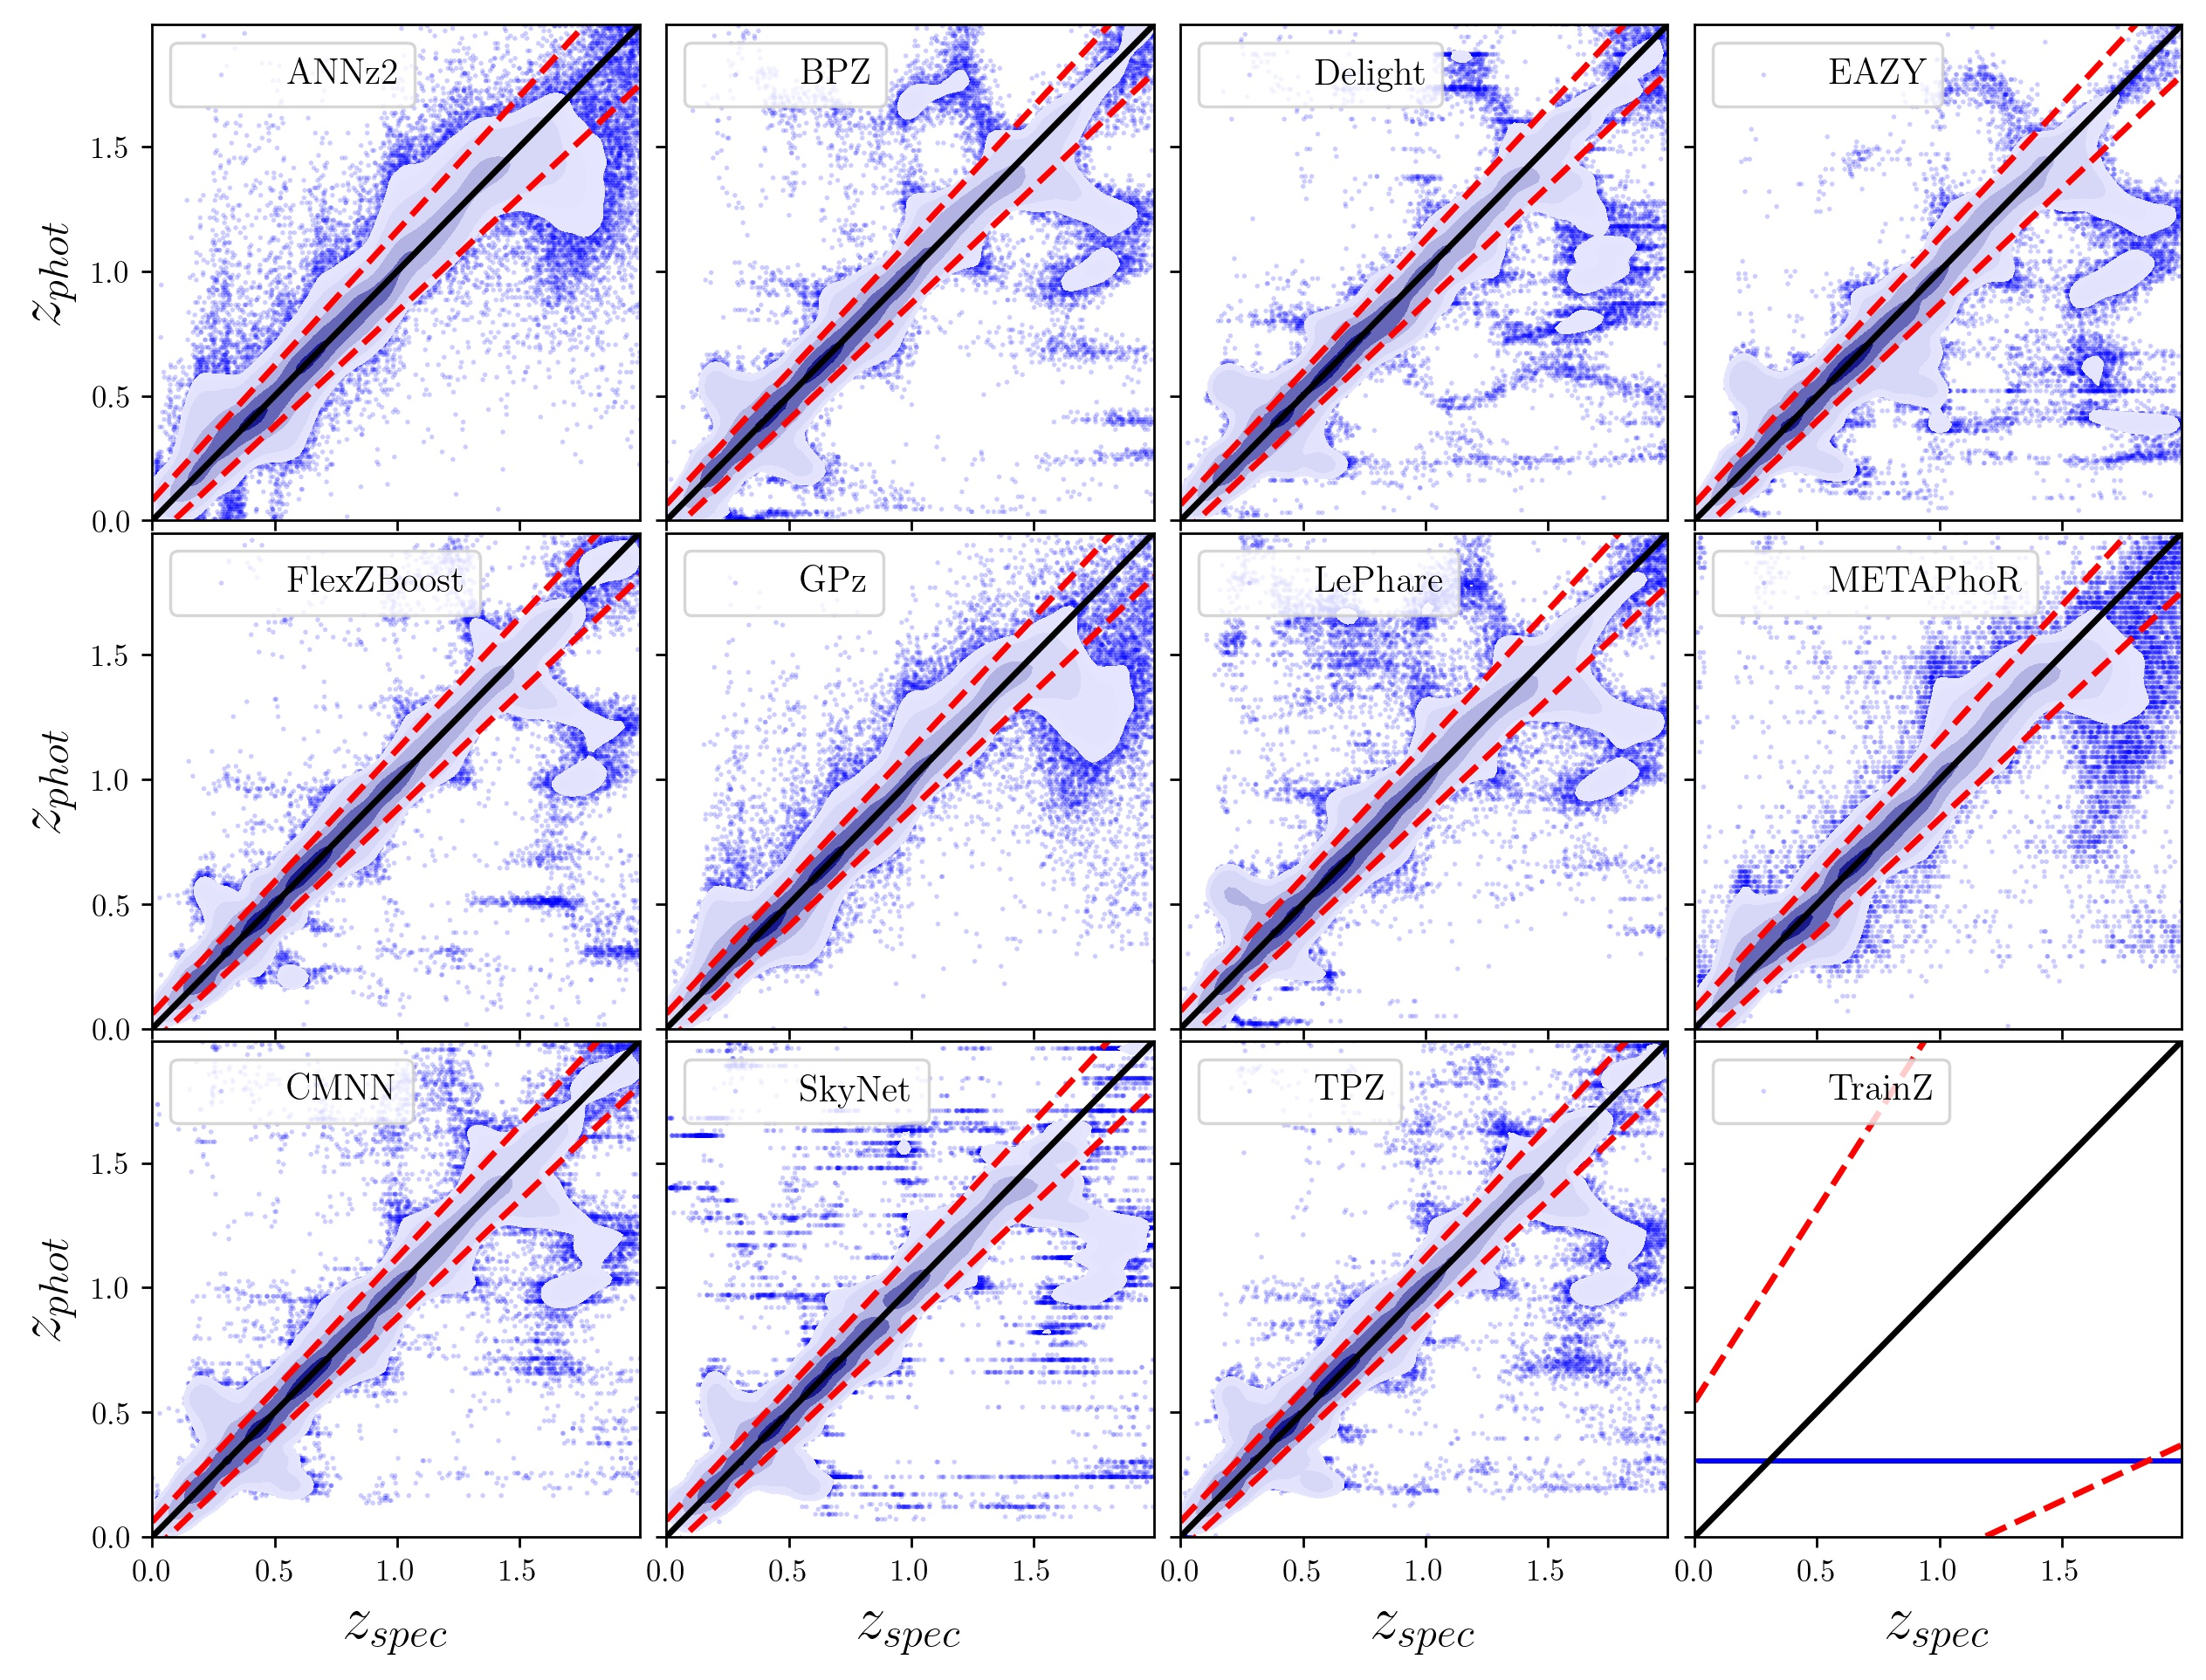
\includegraphics[width=0.8\textwidth]{fig/ZPEAK_szpz_threecolumn_12codes_navy_lowalpha.jpg}\\
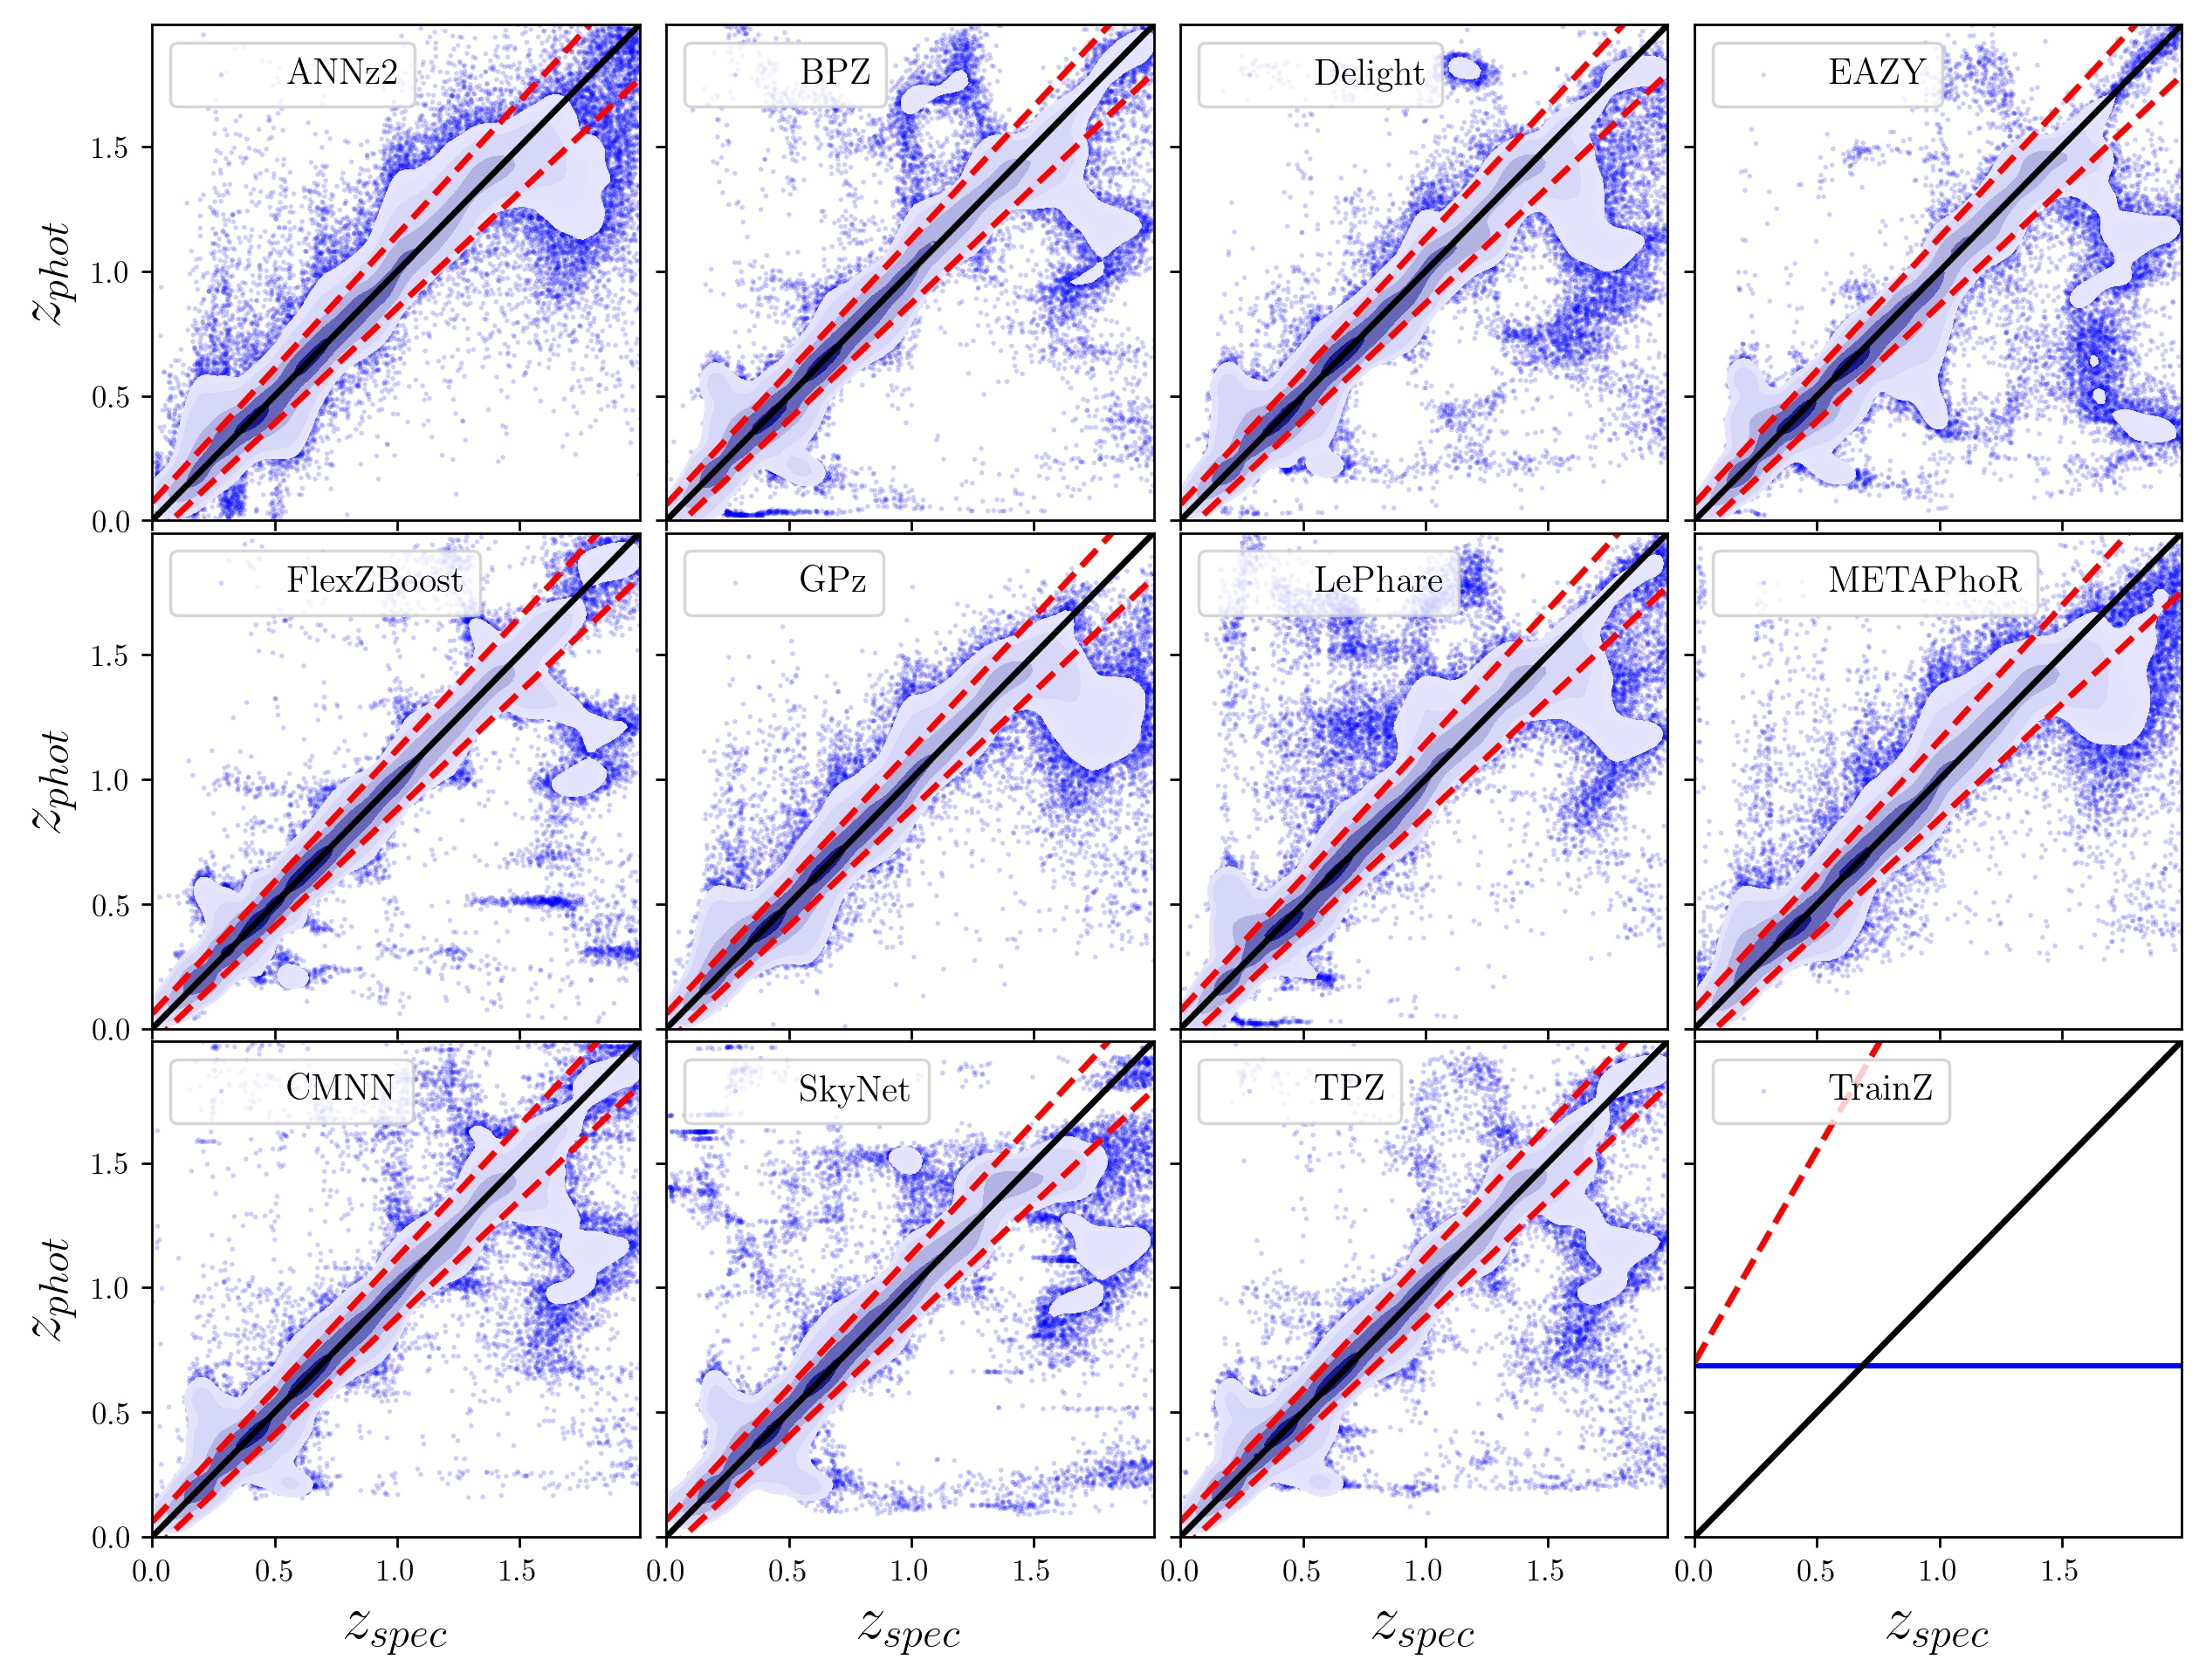
\includegraphics[width=0.8\textwidth]{fig/ZWEIGHT_szpz_threecolumn_12codes_navy_lowalpha.jpg}
\caption{Point estimate photo-z's derived from the posteriors. Top panel shows $z_{PEAK}$, while bottom panel shows $z_{WEIGHT}$.  Point estimate density is represented with fixed density contours, while outliers at lower density are represented by blue points.  While use of point-estimate photo-$z$'s is not recommended, they do make for useful comparative and visual diagnostics.  In the lower-right panel of each plot, the \trainz\ estimator results in identical photo-$z$ estimates at the mode and mean of the training set $N'(z)$ distribution for all galaxies.} \label{fig:pz_pointestimates}
\end{figure*}


\begin{table*}
\begin{center}
\caption{Point estimate statistics}\label{tab:pointestimates}
\begin{tabular}{lcccccc}
\hline
\hline
                 &            & $Z_{PEAK}$  &          &  & $Z_{WEIGHT}$          &\\
\hline
Photo-z Code       & $\frac{\sigma_{IQR}}{(1+z)}$ & median  & \multicolumn{1}{|p{0.75cm}|}{\centering outlier \\fraction} & $\frac{\sigma_{IQR}}{(1+z)}$ & median & \multicolumn{1}{|p{0.75cm}|}{\centering outlier \\fraction}\\
\hline
\textsc{ANNz2}     & 0.0270  &  0.00063  & 0.044      & 0.0244  &  0.000307  & 0.047  \\
\textsc{BPZ}       & 0.0215  & -0.00175  & 0.035      & 0.0215  & -0.002005  & 0.032 \\
\textsc{Delight}   & 0.0212  & -0.00185  & 0.038      & 0.0216  & -0.002158  & 0.038 \\
\textsc{EAZY}      & 0.0225  & -0.00218  & 0.034      & 0.0226  & -0.003765  & 0.029 \\
\textsc{FlexZBoost}& 0.0154  & -0.00027  & 0.020      & 0.0148  & -0.000211  & 0.017 \\
\textsc{GPz}       & 0.0197  & -0.00000  & 0.052      & 0.0195  &  0.000113  & 0.051 \\
\textsc{LePhare}   & 0.0236  & -0.00161  & 0.058      & 0.0239  & -0.002007  & 0.056 \\
\textsc{METAPhoR}  & 0.0264  &  0.00000  & 0.037      & 0.0262  &  0.001333  & 0.048 \\
\textsc{CMNN}        & 0.0184  & -0.00132  & 0.035      & 0.0170  & -0.001049  & 0.034 \\
\textsc{Skynet}    & 0.0219  & -0.00167  & 0.036      & 0.0218  &  0.000174  & 0.037 \\
\textsc{TPZ}       & 0.0161  &  0.00309  & 0.033      & 0.0166  &  0.003048  & 0.031 \\
\hline
\trainz	   & 0.1808  &  -0.2086  & 0.000	  & 0.2335  & 0.022135  & 0.000\\
\end{tabular}
\end{center}
\end{table*}
